\chapter{Medida del rendimiento y perfilado}
\label{chap:medida_rendimiento_perfilado}

\lettrine{T}{ras} plantear la problemática y construir la prueba de concepto, en este capítulo se muestran los resultados de las medidas de rendimiento tanto para los códigos densos como dispersos. Estos resultados se comparan con los que se pueden ver en la literatura ya existente, para comprobar si la red implementada se adhiere a los patrones indicados por ejemplo en la Sección \ref{sec:investigacion_optimizaciones_propuestas}.

\section{Metodología}
\label{sec:metodologia}
La medida del rendimiento de las pruebas de concepto no es tarea trivial. Al ser una simple \textit{\acrlong{poc}} la función \texttt{map\_and\_bias} no está debidamente optimizada con OpenMP. Realizar esta optimización no es difícil, pero quizás sería innecesario cuando lo que se pretende es medir las posibilidades de una aproximación, y no optimizar y trabajar a fondo en ella.

Por esta razón se ha decidido simplemente implementar de forma sencilla la generación de código con las librerías OpenBLAS y librsb, sin añadir OpenMP u optimizaciones mayores en funciones auxiliares. El \textit{overhead} que añade el tratamiento auxiliar de datos es lo suficientemente bajo como para no necesitar paralelización en un entorno de pruebas.

\subsection{Común}
\label{ssec:comun_metodologia}
Para la medida del rendimiento y perfilado se generan dos redes neuronales de un tamaño absurdamente grande, una densa con capas completamente conexas con un anchos tal que \{capa de entrada, $n\:\times\:$capas ocultas, capa de salida\} = \{24, 500, 800, 1000, 1200, 600, 400, 200, 100, 50, 1\}, y otra dispersa con una \textit{sparsity} del 95\% generada a partir del modelo denso. Evidentemente, para el problema que se pretende resolver, estas redes están completamente sobredimensionadas y son cuanto menos inútiles, puesto que debido a su enorme tamaño lo único que aprenden durante el proceso de entrenamiento es a marcar como positivos todos los \textit{inputs}.

Esto, que para un ingeniero en inteligencia artificial sería un enorme fracaso, en este ámbito es algo completamente indiferente, ya que a pesar de la inutilidad de la red creada, esta sigue realizando las cargas de trabajo típicas de una red neuronal adecuada, esto es, multiplica matrices, suma los \textit{bias} y aplica funciones de transferencia.

En ambas ejecuciones se emplean los mismos datos de entrada, que consisten en el fichero \texttt{inupt.txt} generado con la función tratada en el Punto 3 de la Sección \ref{ssec:extraccion_valores}, replicado 100 veces, para obtener $1000 \times 100 = 100000$ datos de entrada.

\subsection{Medida del rendimiento}
\label{ssec:medida_rendimiento_metodologia}
Para la medida del rendimiento se emplea el programa \texttt{hyperfine}\footnote{\url{https://github.com/sharkdp/hyperfine}} y compilaciones de \textit{release} (opción \texttt{-s} o \textit{strip}). Mediante esta herramienta se realizan 15 ejecuciones de las cuales se calcula la media y desviación típica automáticamente, con 3 ejecuciones previas de calentamiento. Siendo un ejemplo de binario generado \texttt{dense.out}, la ejecución del \textit{benchmark} sería tal que:\medskip
\begin{lstlisting}[language=bash]
hyperfine --warmup 3 --runs 15 './dense.out input.txt'
\end{lstlisting}

Tanto las ejecuciones de medición de tiempos como los perfilados se realizan en un equipo Xiaomi Mi Notebook 15 con las características visibles en la Tabla \ref{tb:especificaciones_xiaomi}.
\begin{table}
\centering
\begin{tabular}{|c|c|}
    \hline
    CPU & 11th Gen Intel(R) Core(TM) i7-11370H @ 3.30GHz\\\hline
    RAM & 16 GB @ 3200MHz (Dual Channel)\\\hline
    Sistema & Ubuntu 20.04 - Linux TODO COMPLETAR\\\hline
    CC & gcc 11 TODO CHECKEAR VERSIÓN\\\hline
    OpenBLAS & libopenblas-dev focal, v0.3.8\\\hline
    librsb & librsb-dev focal, v1.2.0.8\\\hline
    oneapi & Intel oneAPI 2022\\\hline
\end{tabular}
\caption{\label{tb:especificaciones_xiaomi}Especificaciones técnicas del equipo de pruebas}
\end{table}


\subsection{Análisis y perfilado}
\label{ssec:analisis_perfilado_metodologia}
Para el análisis y perfilado se emplea el programa Intel Advisor, el cual permite realizar modelos \textit{roofline} de partes individualizadas de programas, incluyendo las funciones de su librería \acrshort{mkl} (\textit{\acrlong{mkl}}). Esto es especialmente útil para perfilar la implementación densa, que emplea funciones de \texttt{cblas} ampliamente utilizadas.

Sin embargo, esta universalidad se pierde con la versión dispersa (\textit{sparse}), ya que se emplean funciones \textit{built-in} de OpenBLAS, así como funciones propias de librsb, lo que hace que cambiar a la \acrshort{mkl} requiera una reprogramación de ciertas líneas del código para poder perfilar las funciones de librería con Intel Advisor. Esto, que inicialmente puede parecer un problema, no lo es tanto si se razona con respecto al \textit{roofline} de la versión densa.

\subsection{Compilación}
\label{ssec:compilacion_metodologia}
Para compilar las versiones densa y dispersa se requiere intercambiar OpenBLAS por la Intel \acrshort{mkl}, así como desactivar el \textit{stripping} del binario para activar los símbolos de depuración (susituir parámetro \texttt{-s} por \texttt{-g}). Esto implica modificar las líneas de compilación genéricas que se pueden encontrar en el fichero \texttt{.ipynb}, tal como se muestra a continuación.

\subsubsection{Código denso}
Para la obtención del \textit{roofline model} de la carga de trabajo, es necesario o bien calcularlo manualmente, o bien emplear alguna herramienta adecuada para ello. Como ya se comenta previamente, se emplea Intel Advisor para el perfilado del código, por lo que es necesario compilar el código denso con una configuración que sustituya OpenBLAS por \acrshort{mkl}. Para esto se puede compilar de las siguientes formas:\medskip
\begin{lstlisting}[language=bash]
# Para una compilación convencional sin depuración con OpenBLAS, sería necesario únicamente ejecutar
gcc -march=native -O3 -s *.c -o dense.out -lm -lcblas       # En Arch Linux
gcc -march=native -O3 -s *.c -o dense.out -lm -lopenblas    # En Ubuntu

# Sin embargo, con propósitos de perfilado con Intel Advisor, en un entorno bash donde se haya realizado `source /opt/intel/oneapi/setvar.sh` se ha de compilar con:
gcc -march=native -O3 -g3 -DMKL_ILP64 -m64 -I"${MKLROOT}/include" *.c -o dense.out -L${MKLROOT}/lib/intel64 -Wl,--no-as-needed -lmkl_intel_ilp64 -lmkl_gnu_thread -lmkl_core -lgomp -lpthread -lm -ldl
\end{lstlisting}

\subsubsection{Código \textit{sparse}}
En este caso, debido al uso de \texttt{librsb} como librería de Sparse BLAS, la herramienta de perfilado y análisis de código Intel Advisor, a pesar de recompilar la librería con \textit{flags} de \textit{debug}, no es capaz de analizar el código de librería. Una adaptación a la librería Intel MKL, a pesar de no ser imposible, no es conveniente. Por esto mismo más adelante en este capítulo se estima el rendimiento y posibilidades de mejora del código disperso, en función a los resultados con respecto al denso. Para compilar el código para \textit{release}, las líneas de compilación son las siguientes:\medskip
\begin{lstlisting}[language=bash]
# Para una compilación convencional sin depuración con OpenBLAS, sería necesario únicamente ejecutar
gcc -march=native -O3 -s *.c -o sparse.out -lm -lrsb -lcblas # En Arch Linux
gcc -march=native -O3 -s *.c -o sparse.out -lm -lrsb -lopenblas  # En Ubuntu
\end{lstlisting}

\section{Medida de rendimiento, perfilado y \textit{roofline model}}
\label{sec:medida_perfilado_roofline}
En esta sección se muestran los resultados obtenidos según la metodología descrita en la sección anterior, así como se razonan los posibles resultados que no se han podido obtener debido a limitaciones en el análisis.

\subsection{Código denso}
Los resultados obtenidos para la red neuronal densa son los siguientes:

\begin{center}
Tiempo $(\overline{t} \pm \sigma)$ = 10,300 s $\pm$ 0,152 s

Rangos (min \ldots\ max) = 10,022 s \ldots\ 10,568 s
\end{center}

Estos resultados se obtienen además realizando un excelente uso de la memoria caché, tal como se muestra en el modelo \textit{roofline} en la Figura \ref{fig:roofline_dense}.

\begin{figure}[h!]
    \centering
    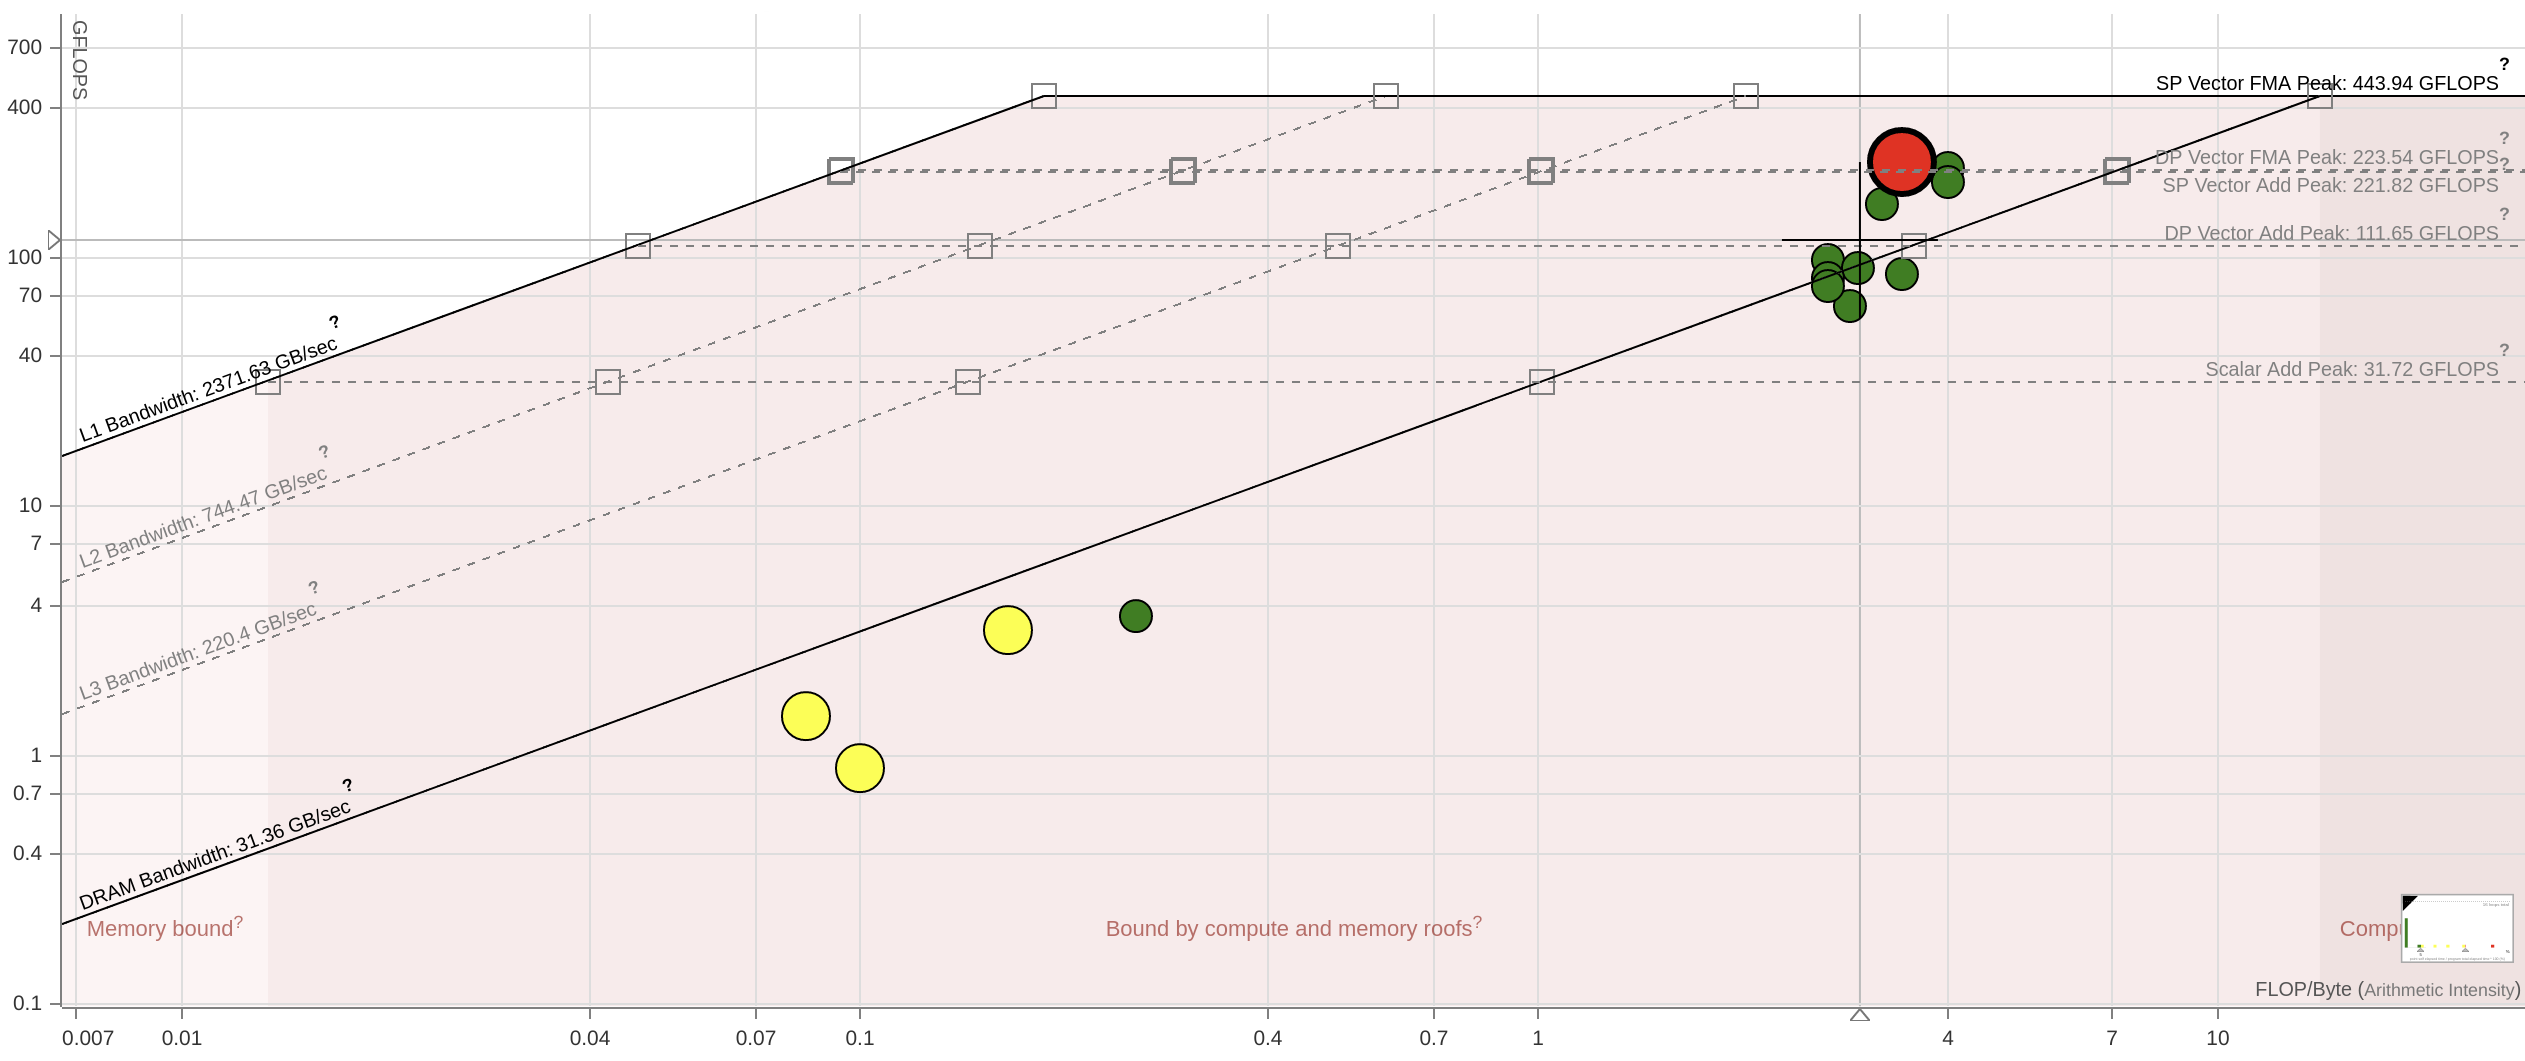
\includegraphics[width=\textwidth]{img/roofline_dense.png}
    \caption{\textit{Roofline model} del código denso}
    \label{fig:roofline_dense}
\end{figure}

Como se puede apreciar en el modelo, el \textit{workload} de interés, que es el que se puede encontrar en la parte superior derecha (coloreado en rojo y verde), corresponde a las funciones \texttt{cblas\_sgemm}. Estas funciones están fuertemente optimizadas y emplean instrucciones AVX512, como se puede observar en los detalles de la carga (Figura \ref{fig:roofline_dense_details}).

Fijándose con atención se pueden ver funciones con un considerablemente menor desempeño en la parte inferior izquierda. Estos puntos corresponden a \texttt{map\_and\_bias} y sucesivas llamadas a otras funciones como \texttt{expf}. Tal como se comenta previamente, una paralelización es sencilla de funciones auxiliares es sencilla. Sin embargo y tal como se puede ver en el modelo, se pueden distinguir perfectamente los componentes de dichas funciones, y siendo el tiempo de ejecución constante para dos redes con las mismas dimensiones, es sencillo discernir qué mejorías vienen causadas por un producto de matrices más eficiente.    

\begin{figure}[h!]
    \centering
    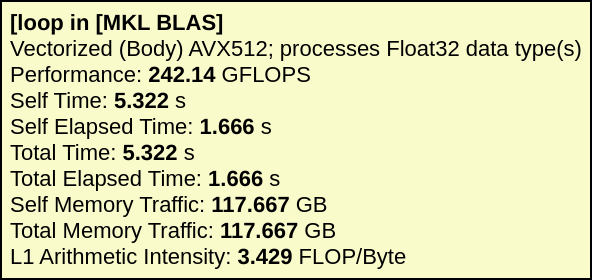
\includegraphics[width=0.5\textwidth]{img/roofline_dense_details.png}
    \caption{Detalles de \texttt{cblas\_sgemm} en el modelo del código denso}
    \label{fig:roofline_dense_details}
\end{figure}

\subsection{Código \textit{sparse}}
Por otro lado, los resultados obtenidos para la red neuronal dispersa son los siguientes:

\begin{center}
Tiempo $(\overline{t} \pm \sigma)$ = 13,862 s $\pm$ 0,710 s

Rangos (min \ldots\ max) = 12,635 s \ldots\ 15,285 s
\end{center}

En este caso, debido al empleo de la librería librsb, el modelo \textit{roofline} no contiene información de utilidad (Figura \ref{fig:roofline_sparse_details}). Esto, que a todas luces es un problema, deja de serlo si se realiza un sencillo razonamiento.

\begin{figure}[h!]
    \centering
    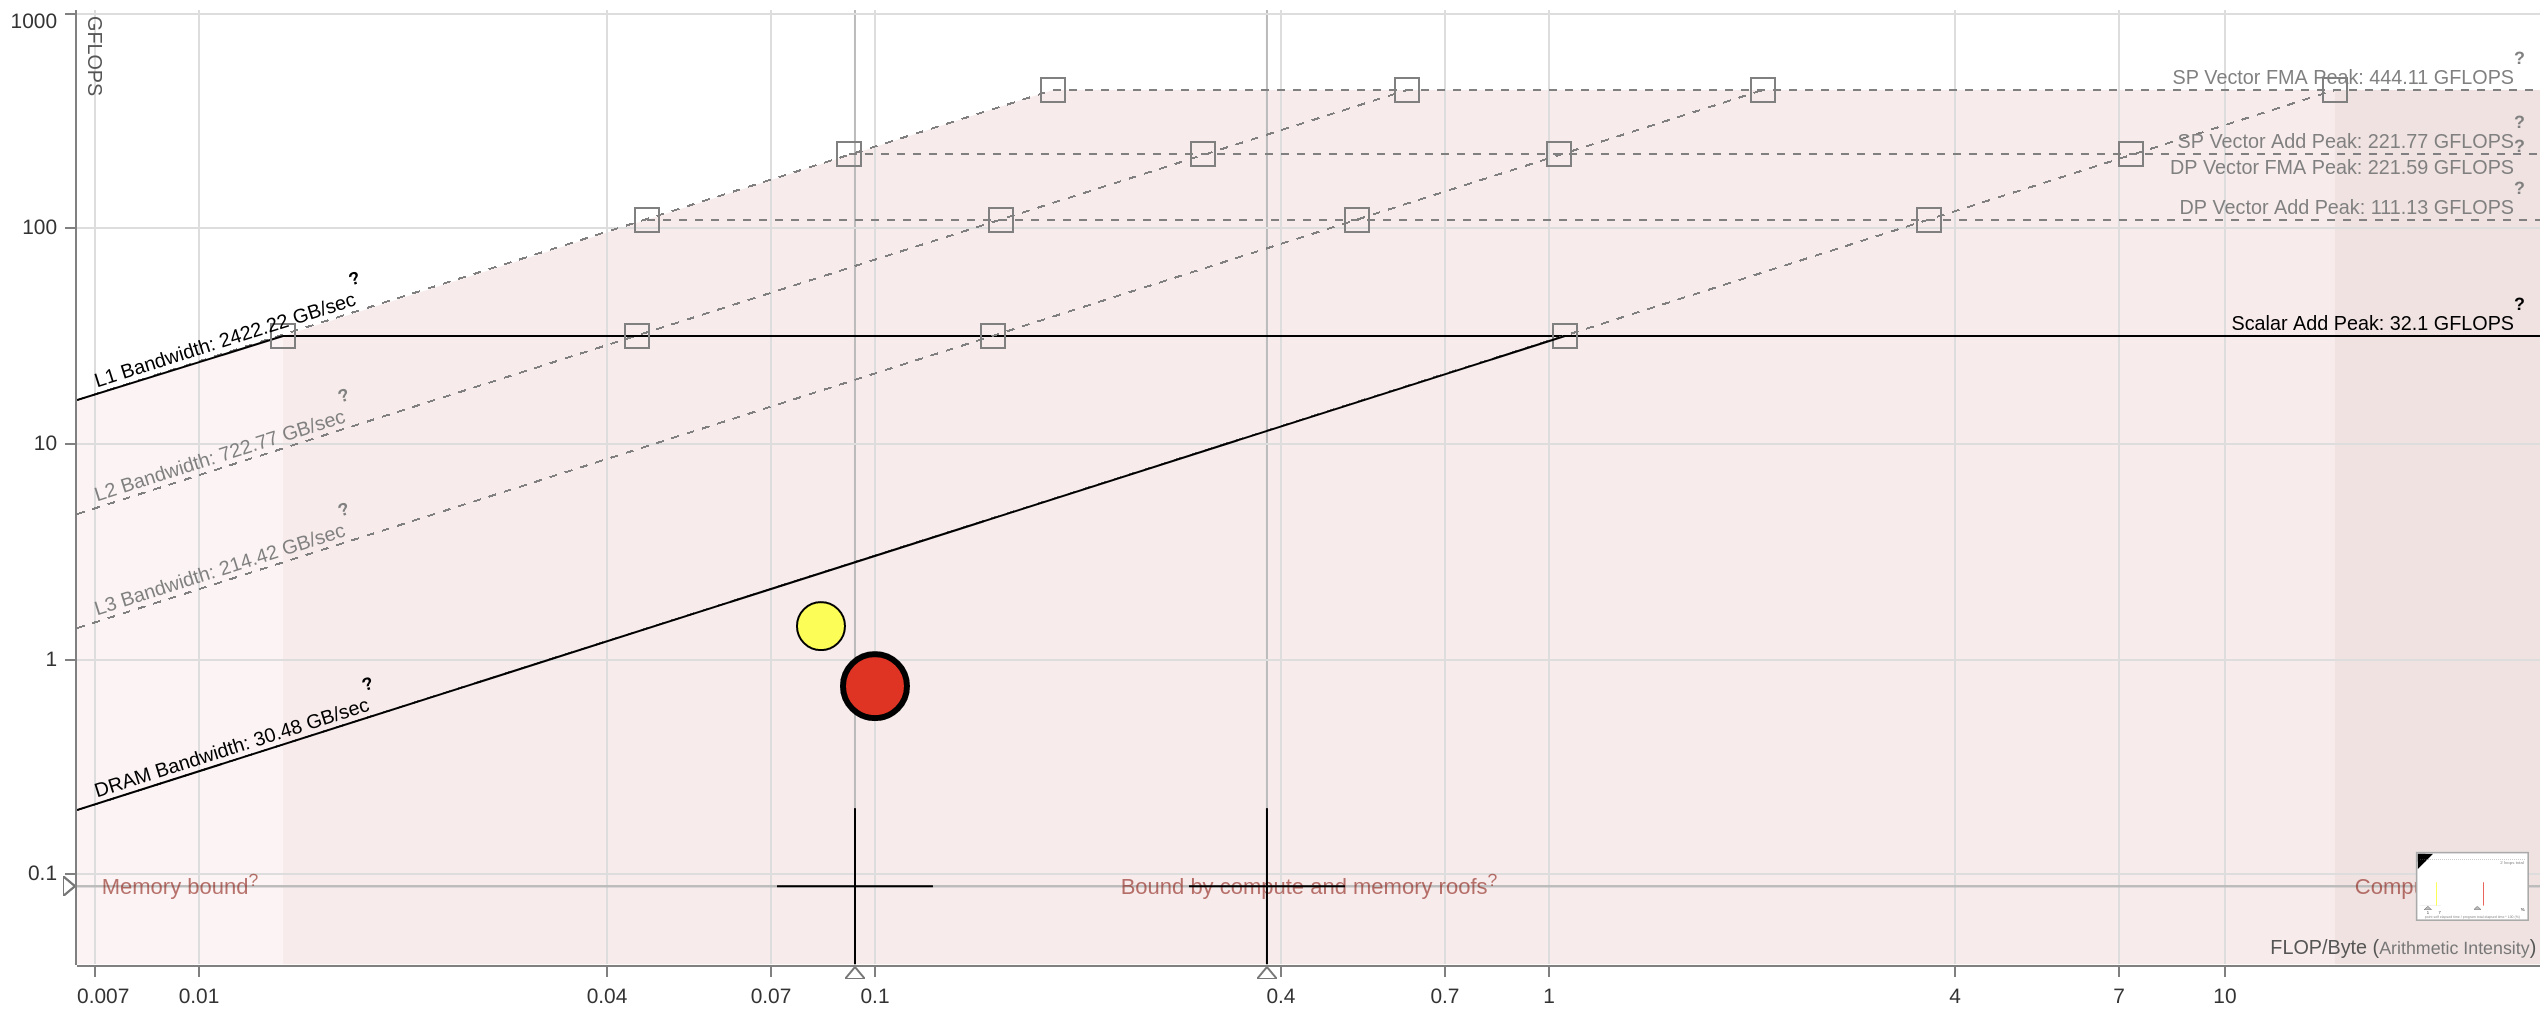
\includegraphics[width=\textwidth]{img/roofline_sparse.png}
    \caption{\textit{Roofline model} del código disperso}
    \label{fig:roofline_sparse_details}
\end{figure}

Teniendo en cuenta que los tiempos de ejecución de una red dispersa al 95\% son \textasciitilde25\% superiores a los de la red completamente conexa, aún teniendo que procesar un 95\% menos de datos, se puede realizar una estimación del número teórico de FLOP necesarios para las operaciones de multiplicación.

\subsubsection{Aproximación teórica}
Sean dos matrices $d \times D$, de dimensiones $m \times n$ y $n \times k$ y la matriz dispersa con una densidad del 50\%, siendo $\#nz$ el número de valores no-cero en la misma:

\begin{gather}
    \begin{pmatrix}
        0 & d_{12}\\
        d_{21} & 0\\
        0 & d_{32}
    \end{pmatrix}	
    \begin{pmatrix}
        D_{11} & \dots\\
        D_{21} & \dots
    \end{pmatrix}
    =
    \begin{pmatrix}
        C_{11} & \dots\\
        C_{21} & \dots\\
        C_{31} & \dots
    \end{pmatrix}
    \label{eq:flops_sparsity_eq}
\end{gather}

Comenzando con $C$ en una región de memoria a ceros, la secuencia de operaciones a realizar sería la siguiente para este ejemplo:

\begin{center}
    $C_{11} \pluseq d_{12} \cdot D_{21}$\\
    $C_{21} \pluseq d_{21} \cdot D_{11}$\\
    $C_{31} \pluseq d_{32} \cdot D_{21}$\\
\end{center}

Esta secuencia \textit{hardcodeada} se repetirá $k$ veces, (el número columnas de $D$ y $C$). Teniendo en cuenta que una operación \texttt{FMA} realiza dos FLOP, se puede concluir que el número de FLOP necesarios para el cálculo de la matriz resultado $C$ será $2 \cdot \#nz \cdot k$.

\subsubsection{Estimación del rendimiento}
Teniendo en cuenta que las matrices dispersas de pesos en el código disperso tienen una densidad del 5\% (o lo que es lo mismo, una \textit{sparsity} del 95\%), desde un punto de vista teórico se puede concluír que se deberían realizar un 95\% menos de operaciones en punto flotante.

Sin embargo esta reducción en el número de operaciones necesarias, debido a múltiples factores como el principio de localidad, estructura interna a la hora de almacenar la matriz, estructuras de control, así como optimizaciones internas de la propia librería, no se corresponde con una disminución del tiempo de ejecución, sino más bien todo lo contrario. Esta reducción en el número de FLOPS no lo es sin embargo en intensidad aritmética, puesto que también se cuenta con menor número de bytes de datos, resultando en un hipotético descenso en el eje $y$ en el modelo.

Por esta razón, el modelo \textit{roofline} resultante, que el programa Intel Advisor es incapaz de generar, se vería similar a lo que se puede observar en la Figura \ref{fig:roofline_sparse_estimado}.

\begin{figure}[h!]
    \centering
    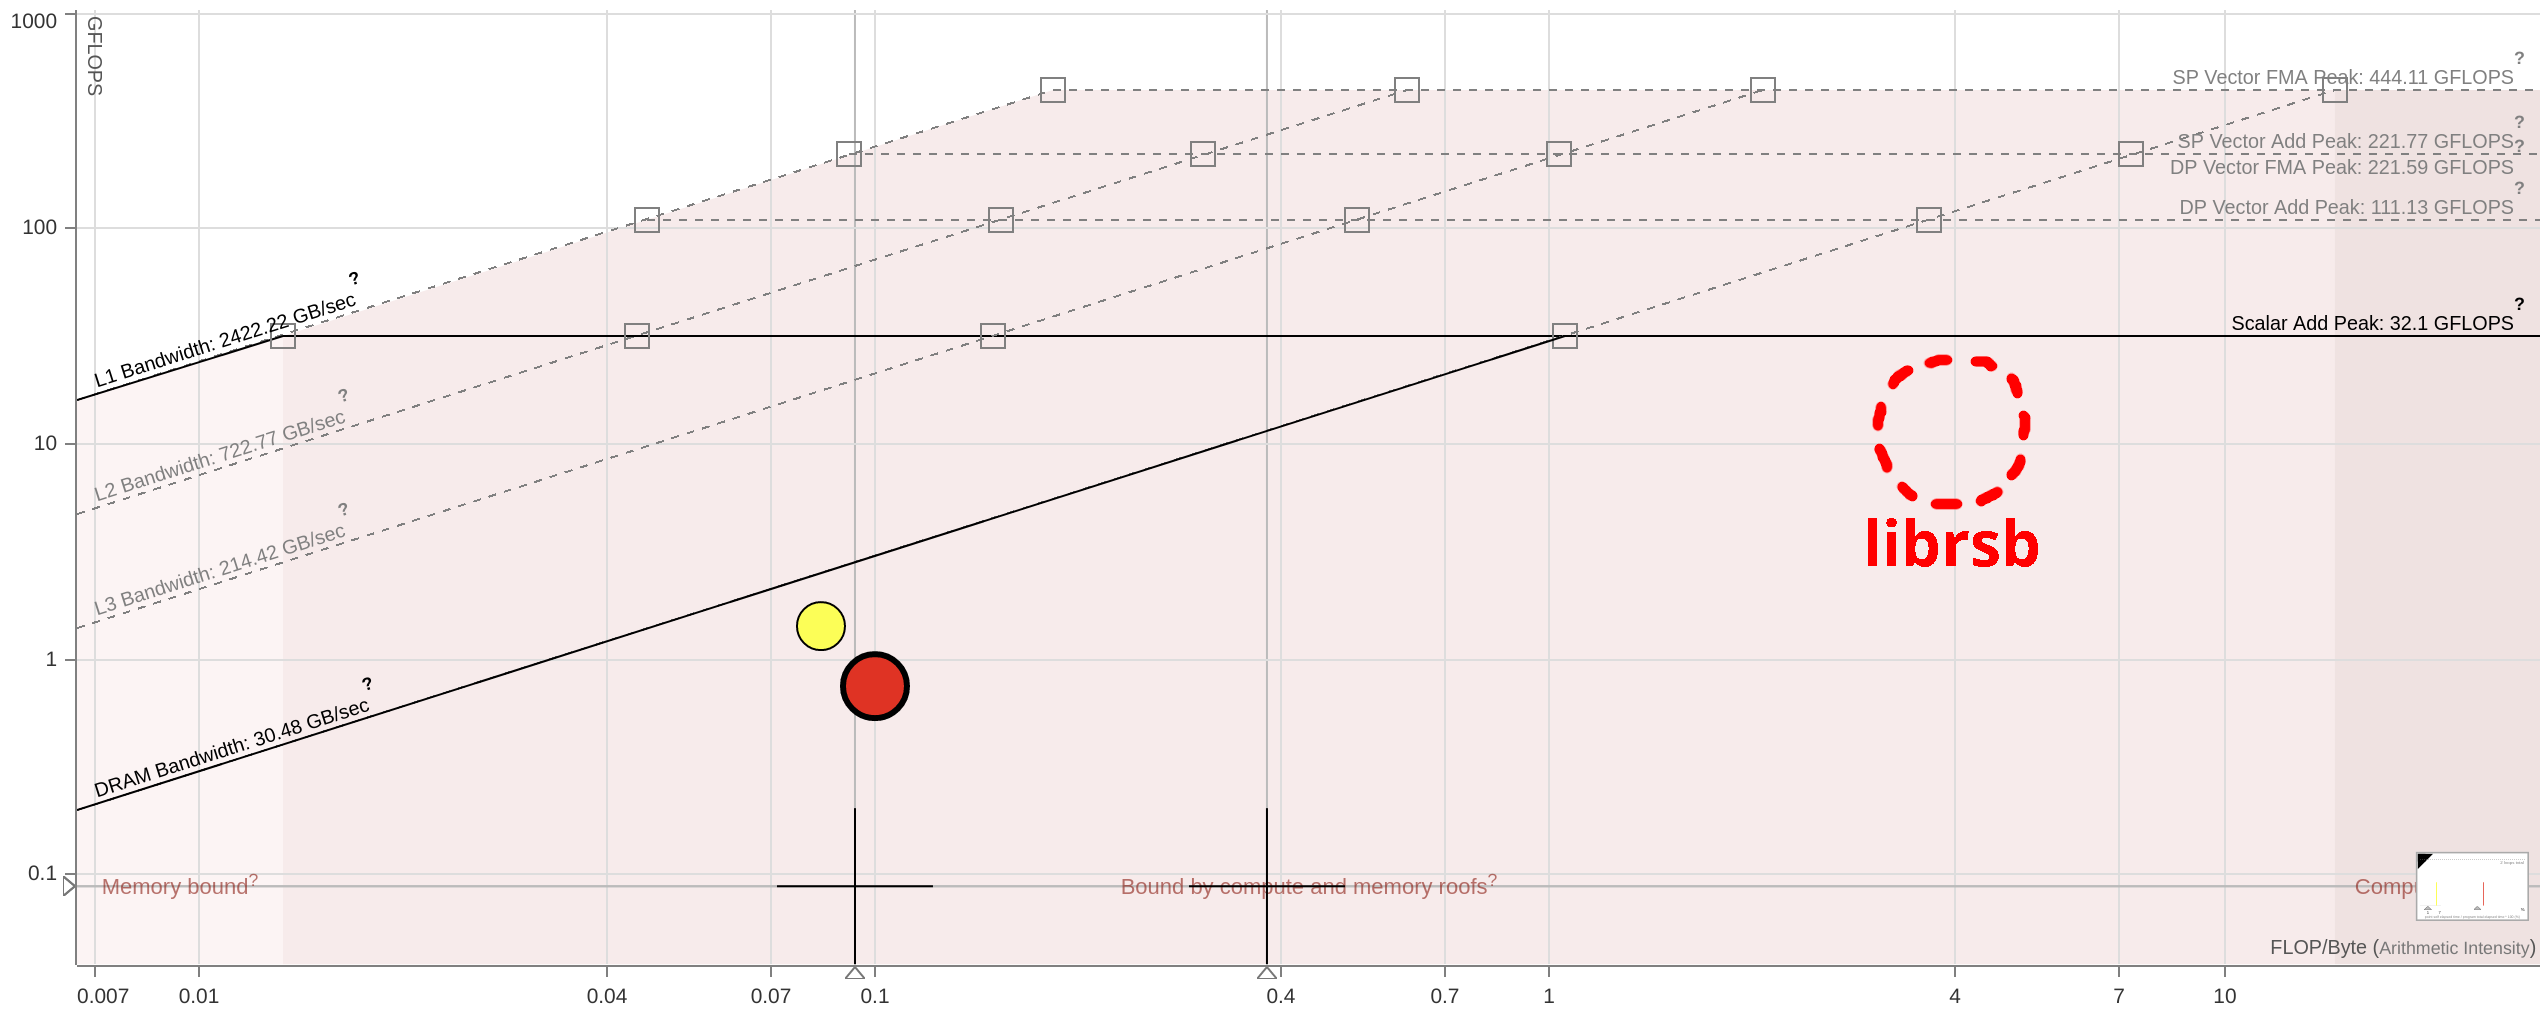
\includegraphics[width=\textwidth]{img/roofline_sparse_estimado.png}
    \caption{Estimación del \textit{roofline model} del código disperso}
    \label{fig:roofline_sparse_estimado}
\end{figure}

Estos decepcionantes resultados, sin embargo, no son tan desalentadores, ya que implica que existe un amplio margen de mejora mediante análisis estático de código y generación de instrucciones FMA y de control \textit{ad-hoc}, que incluso pueden ser vectorizadas mediante el empleo de la herramienta MARTA\footnote{\url{https://github.com/UDC-GAC/MARTA}}.